1- Haciendo uso del montaje indicado en el diagrama esquemático de la figura \ref{fig:offset-y-bias} explicar como medir la tensión de
Offset y como medir la corriente de polarización de cada
.

\begin{figure}[ht]
    \centering
    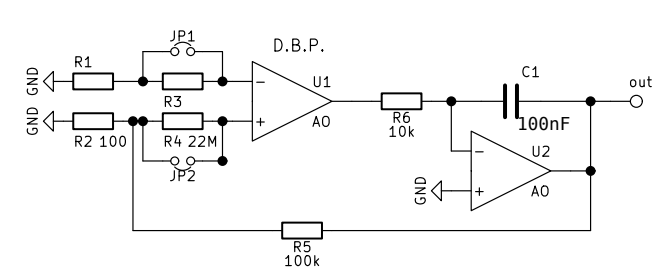
\includegraphics[width=0.5\textwidth]{tension-offset.png}
    \caption{Medición de la tensión Offset y corrientes de polarización}
    \label{fig:offset-y-bias}
\end{figure}

\subsubsection{Tensión Offset}

Para hallar la tension offset  , denotada como $V_{os}$, se va a cerrar los Jumper(JP1) y
(JP2), de esa manera se obtiene la siguiente expresión: 

\begin{equation}
    V_0=\frac{R_5}{R_2}V_{os}
\end{equation}

Se medirá la tensión de salida  $V_o$, por esa razón, se despeja  $V_{os}$, obteniendo de manera indirecta la tension offset.

$V_{os}=\frac{V_o}{1+\frac{R_5}{R_2}}$

\subsubsection{Corriente de Bias}

 Se halla la Corriente de polarización 1 , denotada como $I_{B1}$, se cierra JP 2 y se abre JP 1. Nota: Importante acotación para facilitar los cálculos es que la resistencia  $R_1$ no se tomara en cuenta su caída de tension, debido a que la corriente que pasa por allí es muy pequeña, en consecuencia se desprecia esa tension. Por lo tanto, se obtiene lo siguiente:

 \begin{equation}
    V_o = (V_{os} - I_{B1}R_3)(1 + \frac{R_5}{R_2})
 \end{equation}

 Se medirá la tension de salida  $V_o$. Teniendo todos los demás datos exceptuando $I_{B1}$, es la que se despejara, resultando la siguiente ecuación:


 \begin{equation}
 \boxed{I_{B_1} = \frac{V_{os} \left( 1 + \frac{R_5}{R_2} \right) - V_o}{R_3 \left( 1 + \frac{R_5}{R_2} \right)}}
 \end{equation}

 Se halla asi la corriente de polarización 1, en la medición indirecta de la ecuación 2.

Para hallar la Corriente de polarización 2, denotada como $I_{B2}$, se cierra JP1 y se
abre JP2. Se toma en cuenta la nota anterior, se obtiene:

\begin{equation}
    V_o = \left( V_{os} + I_{B_2} R_4 \right) \left( 1 + \frac{R_5}{R_2} \right)
\end{equation}

Se medirá la tension de salida $V_o$. Teniendo todos los demás datos exceptuando $I_{B2}$, es la que se despejara, resultando la siguiente ecuación:

\begin{equation}
    \boxed{I_{B_2} = \frac{V_o - V_{os} \left( 1 + \frac{R_5}{R_2} \right)}{R_4 \left( 1 + \frac{R_5}{R_2} \right)}}
\end{equation}

Se halla asi la corriente de polarización 2, en la medición indirecta de la ecuación 3.

Al hallar las corrientes de polarización de cada entrada, se puede hacer uso de la siguiente ecuación para conocer la Corriente offset

\begin{equation}
    \boxed{I_{os} = \left| I_{B1} - I_{B2} \right|}
\end{equation}

\subsubsection{Producto del ancho de banda por la ganancia}

2- Mediante el montaje de la figura \ref{fig:gbwp} explique como comprobar que el Producto del Ancho de Banda por la Ganancia
se mantiene

\begin{figure}[ht]
    \centering
    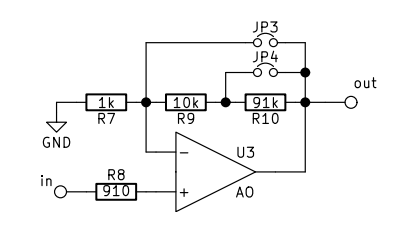
\includegraphics[width=0.5\textwidth]{gbwp.png}
    \caption{Medición de GBWP}
    \label{fig:gbwp}
\end{figure}

En este caso, se verificara que con distintas conexiones de la figura \ref{fig:gbwp}, se mantiene el GBWP, midiendo de manera experimental su frecuencia de corte en las distintas topologías
(variando su frecuencia y observar su atenuación) y poder aproximar su respuesta en frecuencia.

\begin{itemize}
    \item JP3 y JP4 abiertos
    $$A_2 = 1 + \frac{R_{10} + R_9}{R_7} = 102$$
    La primera ganancia es la que se obtiene en la frecuencia mas baja.
    \item JP4 cerrado y JP3 abierto

    $$A_3 = 1 + \frac{R_9}{R_7} = 11$$

    \item JP4 y JP3 cerrado (Buffer)
    $$A_4=1$$

\end{itemize}

\subsubsection{SlewRate, Excursión máxima y corriente de cortocircuito}

\begin{figure}[ht]
    \centering
    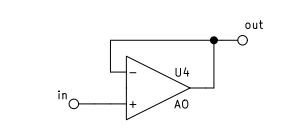
\includegraphics[width=0.5\textwidth]{medicion-sr.png}
    \caption{Medición de SR, Excursión máxima y corriente de cortocircuito}
    \label{fig:medicion-sr}
\end{figure}

\begin{itemize}
    \item SlewRate \\
    Antes de realizar el experimento colocar una frecuencia de 1kHz para luego poder realizar las variaciones. Se realizara con las siguientes instrucciones: Para medir el slew rate utilizando un osciloscopio, se debe conectar el osciloscopio a la salida del amplificador y conilustraciónrlo para mostrar la forma de onda de la señal de salida. Luego, se debe aplicar una señal de entrada triangular al amplificador y ajustar la frecuencia de la señal para que este dentro del rango de operación del amplificador. A continuación, se debe medir el tiempo que tarda la señal de salida en cambiar desde el 10 \% al 90 \% de su valor máximo, y utilizar esta información para calcular el slew rate utilizando la siguiente formula:

    $$SR = \frac{\Delta V}{\Delta t}$$

    Donde SR es el slew rate, $\Delta V$ es el cambio en la tension de salida y $\Delta V$ es el tiempo que tarda la señal de salida en cambiar desde el 10 \% al 90 \% de su valor máximo. Es importante tener en cuenta que el slew rate puede variar dependiendo de la frecuencia de la señal de entrada, por lo que se deben realizar mediciones en diferentes frecuencias para obtener una medida precisa del slew rate.

    \begin{ilustracion}[ht]
        \centering
        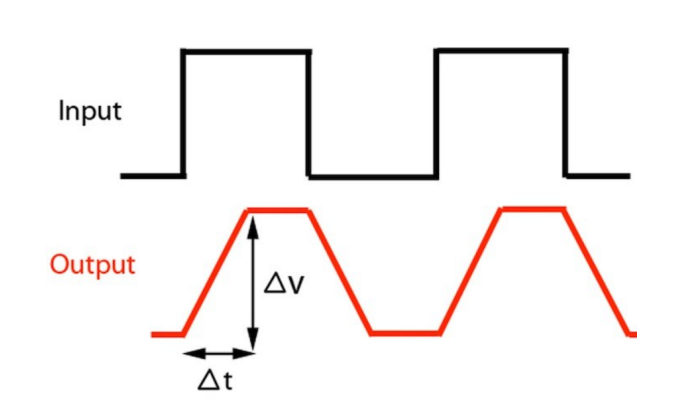
\includegraphics[width=0.5\textwidth]{senales-retardo.png}
        \caption{Comparación tiempo de retardo entre señal de entrada y de salida debido al S.R de la variación de la frecuencia}
        \label{ilus:comparacion-funciones-sr}
    \end{ilustracion}

    \item Limites máximo de excursion
    Se sube solo el voltaje para observar la señal de salida cuando esta se distorsione, recordar que se debe colocar nuevamente la frecuencia en 1KHz.

    \item Corriente de corto circuito
    \begin{ilustracion}[ht]
        \centering
        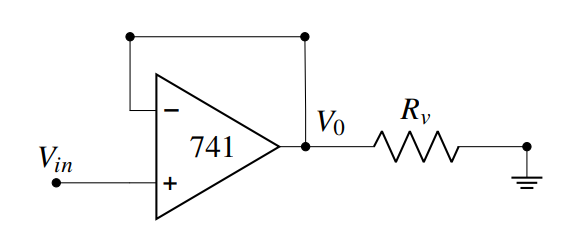
\includegraphics[width=0.5\textwidth]{medicion-corriente-cortocircuito.png}
        \caption{Medición de corriente en corto circuito}
        \label{ilus:medicion-corriente-cortocircuito}
    \end{ilustracion}
    Para la corriente de cortocircuito, se puede usar la técnica de "Resistencia de Carga virtual",esto es colocar una resistencia virtual en serie con la carga real del circuito, lo que permite medir la caída de tension a traves de la carga virtual.

    La resistencia debe ser lo mas pequeña posible entre $1\Omega$ y $10\Omega$, mido la tension sobre esta resistencia y por ley de Ohm se puede hallar la corriente de cortocircuito


\end{itemize}